%-*- coding: iso-latin-1 -*-
%\PassOptionsToPackage{dvipsnames}{xcolor} % for compatibility with tikzsymbols
\documentclass[french,11pt,openany]{book}
\usepackage{babel}
\DecimalMathComma
% Emacs: to save in encoding iso-latin-1:
% C-x C-m f
% iso-latin-1

% aspell --lang=fr --encoding='iso-8859-1' -t check selection-modele.tex

% Fonts
\usepackage[latin1]{inputenc}
\usepackage[T1]{fontenc}
\usepackage{gentium}

% SI units
\usepackage{siunitx}

\usepackage{textcomp}


% TODO
\usepackage[dvipsnames]{xcolor}
\newcommand{\todo}[1]{{\color{BrickRed}{TODO~#1}}}
\newcommand{\rewrite}[1]{{\color{RoyalBlue}{#1}}}
\newcommand{\erratum}[1]{{\color{Red}{ERRATUM : ~#1}}}



%%%% TABLES & FIGURES %%%%%%%%%%%%%%%%%%%%%%%%%%%%%%%%%%%%%%%%%%%%%%%%%%%
\usepackage{graphicx}
\usepackage{subcaption} % Side-by-side figures
\usepackage{tikz}

\usepackage{multirow}
% Table becomes Tableau
\usepackage{caption}
\captionsetup{labelfont=sc}
\def\frenchtablename{Tableau}
%%%%%%%%%%%%%%%%%%%%%%%%%%%%%%%%%%%%%%%%%%%%%%%%%%%%%%%%%%%%%%%%%%%%%%

\usepackage[colorlinks=true,urlcolor=MidnightBlue,linkcolor=black,citecolor=black]{hyperref}

%%%% GEOMETRY AND SPACING %%%%%%%%%%%%%%%%%%%%%%%%%%%%%%%%%%%%%%%%%%%%%%%
\usepackage[tmargin=2cm,bmargin=2cm,lmargin=3cm,footnotesep=1cm]{geometry}

\usepackage{changepage}

% Vertical spaces
\parskip=1ex\relax % space between paragraphs (incl. blank lines)
\usepackage{enumitem}
\setlist[itemize]{itemsep=0pt,topsep=0pt}
\setitemize{itemsep=1pt} % space between items

\usepackage{titlesec}
\titlespacing{\paragraph}{%
  0pt}{%              left margin
  0.5\baselineskip}{% space before (vertical)
  1em}%               space after (horizontal)

\titlespacing*{\section}{0pt}{10pt}{0pt}

\titleclass{\part}{top}
\titleformat{\part}[display]
  {\normalfont\huge\bfseries}{\centering\partname\ \thepart}{5pt}{\Huge\centering}
\titlespacing*{\part}{0pt}{50pt}{40pt}

\titleclass{\chapter}{straight}
\titlespacing*{\chapter}{0pt}{50pt}{30pt}
\titleformat{\chapter}%[display]
{\normalfont\huge\bfseries}{\chaptertitlename\ \thechapter}{15pt}{\huge}

\usepackage[all]{nowidow}
%%%%%%%%%%%%%%%%%%%%%%%%%%%%%%%%%%%%%%%%%%%%%%%%%%%%%%%%%%%%%%%%%%%%%%

  

% Mathematical symbols
\input{contents/notations}



%%% CODE LISTINGS %%%%%%%%%%%%%%%%%%%%%%%%%%%%%%%%%%%%%%%%%%%%%%%%%%%%
\usepackage{listings}
\lstset{%
  frame=single,                    % adds a frame around the code
  % numbers=left,                    % where to put the line-numbers; possible values are (none, left, right)
  % numbersep=5pt,                   % how far the line-numbers are from the code
  tabsize=2,                       % sets default tabsize to 2 spaces
  columns=flexible,                % doesn't add spaces to make the line fit the whole column
  basicstyle=\ttfamily,             % use monospace
  keywordstyle=\color{MidnightBlue},
  commentstyle=\color{Gray},
  stringstyle=\color{BurntOrange},
  showstringspaces=false,
  %identifierstyle=\color{MyBlue},
  %procnamekeys={def,class}
}
%%%%%%%%%%%%%%%%%%%%%%%%%%%%%%%%%%%%%%%%%%%%%%%%%%%%%%%%%%%%%%%%%%%%%%



%%% ENVIRONNEMENTS %%%%%%%%%%%%%%%%%%%%%%%%%%%%%%%%%%%%%%%%%%%%%%%%%%%
\makeatletter
\def\forcedefenv#1{%%
\global\expandafter\let\csname#1\endcsname\relax
\global\expandafter\let\csname end#1\endcsname\relax
}

% Environnement "plusloin".
%
\forcedefenv{plusloin}
\newenvironment{plusloin}[1][Pour aller plus loin]{\par\medbreak
\noindent\makebox[\textwidth]{\hrulefill\quad#1\quad\hrulefill}\par\nobreak
\@afterheading
\def\labelitemi{\textbullet}
\begin{itemize}
\setlength{\itemsep}{1ex}}{\end{itemize}\par\nobreak\noindent\makebox[\textwidth]{\hrulefill}\nobreak\par}

% Environnement "attention". 
%
\forcedefenv{attention}
\newenvironment{attention}
{\par \noindent\rule[\baselineskip]{\textwidth}{1pt}\vspace{-\baselineskip}
{\centering{\textbf{Attention}}\par}
}
{\par \noindent\rule[\baselineskip]{\textwidth}{1pt}\vspace{-\baselineskip}\par}


% Environnement "encadre". 
%
\forcedefenv{encadre}
  \newenvironment{encadre}[1]{\par\medbreak
  \noindent\fbox{\parbox{\linewidth}{
{\ifx#1\relax\else{\strut#1\par\nobreak}\vspace*{3mm}\par\nobreak\fi}
    }}}

\forcedefenv{exemple}
\newenvironment{exemple}
{\par 
\begin{adjustwidth}{2em}{2em}
\noindent\rule{10pt}{0.4pt} \; \textbf{Exemple} \; \hrulefill \par}
{\par \noindent\rule[\baselineskip]{\textwidth-4em}{0.4pt}\vspace{-\baselineskip}\par
\end{adjustwidth}}

\forcedefenv{answer}
\newenvironment{answer}
{\par\noindent
  \textbf{R�ponse} \hrulefill \par}
{\par \noindent\rule[\baselineskip]{\textwidth}{0.4pt}\vspace{-\baselineskip}\par}


% Environnement "remarque". 
\forcedefenv{remarque}
\newenvironment{remarque}[1][\relax]{\par\medbreak
\noindent\makebox[\textwidth]{\hrulefill\quad Remarque\quad\hrulefill}\par\nobreak
\ifx#1\relax\else{\centering\bfseries\large \strut#1\par\nobreak}\vspace*{3mm}\par\nobreak\fi
\@afterheading 
}{\par\nobreak\par\noindent\makebox[\textwidth]{\hrulefill%\quad Fin Encart\quad\hrulefill
}\nobreak\bigbreak}
\makeatother
%%%%%%%%%%%%%%%%%%%%%%%%%%%%%%%%%%%%%%%%%%%%%%%%%%%%%%%%%%%%%%%%%%%%%%




\begin{document}

% Vertical spacing above/before equations
\setlength{\abovedisplayskip}{5pt}
\setlength{\belowdisplayskip}{3pt}


\renewcommand{\bibname}{}


\begin{center}
  
  \hfill

  \vfill
  
  \LARGE 
  ECUE21.2 Science des donn�es (DATA)\\ 
  
  \Large
  Chlo�-Agathe Azencott (CBIO) \\

  Printemps 2021 -- Mines ParisTech

  \vfill

  \large
  \textbf{Comp�tences} 


  \begin{tabular}[h]{|p{0.025\textwidth}|p{0.975\textwidth}|}
    \hline
    C1 & Ma�triser des m�thodes statistiques usuelles permettant de traiter convenablement des cas simples d'analyse de donn�es \\ \hline
    C2 & Ma�triser des m�thodes usuelles d'exploration des donn�es \\ \hline
    C3 &  Conna�tre les limites d'applications des m�thodes vues en cours \\ \hline
    C4 & Pouvoir se r�f�rer � un cas d'application avec des donn�es r�elles en lien avec une discipline autre que celle de l'analyse des donn�es \\ \hline
    C5 & Savoir �valuer la complexit� num�rique de quelques algorithmes \\ \hline
    C6 & Conna�tre des m�thodes d'apprentissage statistique (machine learning) supervis� et des m�thodes d'apprentissage statistique non supervis� \\ \hline
    C7 & Savoir valider et s�lectionner un mod�le statistique \\ \hline
  \end{tabular}

  \vfill

\end{center}
\clearpage

\tableofcontents
\clearpage


\chapter{Introduction}
\input{contents/intro}

\part{Notions de statistique}
\chapter{Statistique descriptive}
\input{contents/stat_descriptive}
\clearpage 

\chapter{Estimation}
%-*- coding: iso-latin-1 -*-
\label{chap:estimation}

\paragraph{Notions :} �chantillon al�atoire, estimateur, estimation, biais d'un
estimateur, convergence d'un estimateur, estimation par maximisation de la
vraisemblance, estimation de Bayes.
\paragraph{Objectifs p�dagogiques :}
\begin{itemize}
\setlength{\itemsep}{3pt}
\item Choisir un estimateur, en particulier en d�terminant des propri�t�s
  telles que son biais ou sa pr�cision.
\item Proposer un estimateur, en particulier par maximisation de la
  vraisemblance.
\end{itemize}


\section{Inf�rence statistique}
Alors que la statistique descriptive se contente de \textit{d�crire} une
population ou un �chantillon de celle-ci, l'inf�rence statistique cherche �
tirer des conclusions sur une population � partir de l'�tude d'un �chantillon
de celle-ci. 

\section{�chantillonnage}
\label{ref:echantilonnage}

Lorsque la population � �tudier est trop grande pour qu'il soit possible
d'observer chacun de ses individus, on �tudie alors une partie seulement de la
population. Cette partie est appel�e \textbf{�chantillon}. On parle alors de
\textbf{sondage}, par opposition � un \textbf{recensement}, qui consiste �
�tudier tous les individus d'une population.

\paragraph{Hypoth�ses de l'�chantillonnage} Pour tirer parti d'un �chantillon,
nous allons avoir besoin des hypoth�ses suivantes :
\begin{itemize}
\item La taille de la population est infinie ;
\item Les variables mesur�es sur la population peuvent �tre consid�r�es comme
  des variables al�atoires, dont les mesures sont des r�alisations. Les lois de
  probabilit� suivies par ces variables peuvent appartenir � une famille connue
  (e.g. loi gaussienne, loi de Poisson, etc.) ou �tre totalement
  inconnues. Dans le premier cas, on parlera de \textbf{statistique
    inf�rentielle param�trique} ; dans le deuxi�me, de \textbf{statistique
    inf�rentielle non-param�trique}.
\end{itemize}

\paragraph{Objectifs de la statistique inf�rentielle} La statistique
inf�rentielle a alors pour but d'\textbf{identifier les lois de probabilit� de ces
  variables al�atoires.} Cela peut prendre les
formes suivantes :
\begin{itemize}
\item L'\textbf{estimation}, qui permet de d�terminer les param�tres des lois (param�tre
  $p$ d'une loi de Bernoulli, indice et param�tre d'�chelle d'une loi Gamma) ou
  certaines de leurs caract�ristiques (esp�rance, variance, moments d'ordre
  sup�rieur, quartiles, etc.). C'est le sujet de ce chapitre.
\item Les \textbf{tests d'hypoth�se}, qui permettent d'infirmer ou de confirmer des
  hypoth�ses faites sur ces lois, leurs param�tres ou leurs
  caract�ristiques. Il s'agit par exemple de d�cider s'il est plausible que
  l'esp�rance d'une variable soit sup�rieure � une certaine valeur ; ou qu'une
  variable suive une loi normale. C'est le sujet du chapitre~\ref{chap:tests}.
\end{itemize}

\paragraph{�chantillonnage al�atoire}
Dans la suite de ce chapitre, nous allons consid�rer que l'�chantillon obtenu
par sondage est obtenu par \textbf{�chantillonnage al�atoire simple} : on
pr�l�ve des individus dans la population au hasard, sans remise. Chaque
individu de la population a la m�me probabilit� $1/N$ d'�tre pr�lev�, o� $N$
est la taille de la population (on rappelle que $N \rightarrow \infty$) et les 
individus sont pr�lev�s ind�pendamment les uns des autres.

\paragraph{Autres techniques d'�chantillonnage} D'autres techniques
d'�chantillonnage sont possibles, comme l'�chantillonnage al�atoire
\textit{stratifi�}, dans lequel la population est partitionn�e en strates selon
une caract�ristique (par exemple, par tranche d'�ge), et l'�chantillon est
obtenu en proc�dant � un �chantillonnage al�atoire simple dans chacune des
strates. On obtient ainsi pour chaque strate un �chantillon de taille
proportionnelle � la taille de la strate dans la population. En d'autres
termes, les individus n'ont pas tous la m�me probabilit� d'�tre tir�s :
celle-ci d�pend de la taille de la strate � laquelle ils appartiennent.

\paragraph{Repr�sentativit�} Avant de tirer des conclusions d'un �chantillon
al�atoire, il est important de s'assurer que celui-ci est repr�sentatif de la
population �tudi�e. Par exemple, les premi�res �tudes cliniques d�montrant
l'efficacit� de l'aspirine pour r�duire le risque d'infarctus du myocarde chez
les patients � risque portaient sur des �chantillons compos�s principalement
d'hommes ; ce n'est que bien plus tard que la communaut� m�dicale a r�alis� que
l'efficacit� est bien moindre chez les femmes.

\paragraph{�chantillon al�atoire et �chantillon} Deux �chantillons $(x_1, x_2, \dots, x_n)$ et
$(x^\prime_1, x^\prime_2, \dots, x^\prime_n)$ de tailles identiques $n$ de la
m�me population seront donc diff�rents. On mod�lise cette variabilit� en
consid�rant que les individus $x_i$ et $x^\prime_i$ sont la r�alisation
d'une m�me variable al�atoire $X_i.$ $(X_1, X_2, \dots, X_n)$ est un vecteur
al�atoire dont les composantes sont ind�pendantes et identiquement
distribu�es (iid).
\begin{itemize}
\item $(X_1, X_2, \dots, X_n)$ est appel� \textbf{�chantillon al�atoire} ;
\item $(x_1, x_2, \dots, x_n)$ et $(x^\prime_1, x^\prime_2, \dots, x^\prime_n)$
  sont deux �chantillons, c'est-�-dire deux \textit{r�alisations} de cet
  �chantillon al�atoire.
\end{itemize}

Un indicateur statistique de l'�chantillon est alors la r�alisation d'une
variable al�atoire fonction de l'�chantillon al�atoire.

\begin{exemple} La moyenne d'un �chantillon,
$\bar{x} = \frac1n \sum_{i=1}^n x_i,$ est la r�alisation d'une variable
al�atoire $M_n$ d�finie par
\[
  M_n = \frac1n \sum_{i=1}^n X_i,
\]
qui est une fonction de l'�chantillon al�atoire $(X_1, X_2, \dots, X_n)$.
\end{exemple}

\section{Estimation ponctuelle}
Soit $(\Omega, \Acal, \PP)$ un espace probabilis�, $E$ un espace mesurable, et
$X$ une variable al�atoire � valeurs dans $E$. En pratique, dans la suite de ce
chapitre, nous consid�rerons des variables al�atoires r�elles ($E = \RR$ ou une
partie de $\RR$ telle que $\RR_+$ ou $\NN$), mais les id�es qui y sont
pr�sent�es peuvent �tre �tendues � $\RR^d$ ou � des espaces plus sophistiqu�s.

Soit $(X_1, X_2, \dots, X_n)$ un �chantillon al�atoire. Les $X_i$ sont
ind�pendantes et identiquement distribu�es, de m�me loi $\PP_X$ que $X.$ Soit
$(x_1, x_2, \dots, x_n)$ un �chantillon, autrement dit une r�alisation de cet
�chantillon al�atoire. Soit enfin $\theta \in \RR$ une quantit� d�terministe
(autrement dit, il ne s'agit pas d'une variable al�atoire), qui d�pend
uniquement de $\PP_X.$ Le but de l'estimation ponctuelle est d'approcher au
mieux la valeur de $\theta$.

Par exemple, si l'on fait l'hypoth�se que $X$ suit une loi exponentielle (nous
sommes donc dans un contexte de statistique inf�rentielle param�trique),
$\theta$ peut �tre le param�tre de cette loi, mais aussi un de ses moments, un
quantile, etc.


\subsection{D�finition d'un estimateur}
On appelle \textbf{estimateur} de $\theta$ une statistique de l'�chantillon
al�atoire $(X_1, X_2, \dots, X_n),$ c'est � dire une variable al�atoire
fonction de $(X_1, X_2, \dots, X_n) :$ un estimateur $\Theta_n$ de $\theta$
peut �tre d�fini par 
\[
  \Theta_n = g(X_1, X_2, \dots, X_n), \qquad g: E^n \rightarrow \RR.
\]

�tant donn� un �chantillon $(x_1, x_2, \dots, x_n)$ de $X$, on appelle
\textbf{estimation} de $\theta$ la valeur
\[
  \thetahat_n = g(x_1, x_2, \dots, x_n) \in \RR,
\]
qui est donc une r�alisation de $\Theta_n$.

\paragraph{R�sum�}
�tant donn� une variable al�atoire r�elle $X$ � valeurs dans $E,$ un entier
$n \in \NN^*$, et une valeur $\theta$ � estimer qui ne d�pend que de la loi de
$X,$
\begin{itemize}
\item un �chantillon al�atoire $(X_1, X_2, \dots, X_n)$ est un vecteur
  al�atoire, dont les composantes sont iid de m�me loi que $X$ ;
\item un �chantillon $(x_1, x_2, \dots, x_n) \in \RR^n$ est une r�alisation de
  ce vecteur al�atoire ;
\item un estimateur de $\theta$ est une variable al�atoire $\Theta_n$ fonction
  de $(X_1, X_2, \dots, X_n)$ : \\ $\Theta_n = g(X_1, X_2, \dots, X_n)$, avec $g: E \rightarrow \RR$ ;
\item une estimation de $\theta$ est une r�alisation $\thetahat_n$ de
  $\Theta_n$ : $\thetahat_n = g(x_1, x_2, \dots, x_n) \in \RR.$
\end{itemize}

\subsection{Exemple : estimation de la moyenne par la moyenne empirique}
Consid�rons maintenant que $X$ est de carr� int�grable ($X \in \Lcal^2$),
d'esp�rance $m$ et de variance $\sigma^2$.

La \textbf{moyenne empirique} de $X$ est une variable al�atoire $M_n$, d�finie
par
\begin{equation}
  M_n = \frac1n \sum_{i=1}^n X_i.
  \label{eq:moyenne_empirique}
\end{equation}

$M_n$ est un estimateur de $m$ : �tant donn� un �chantillon
$(x_1, x_2, \dots, x_n),$ la valeur $\hat{m}_n = \frac1n \sum_{i=1}^n x_i$ est
une estimation de $m$.

� ce stade, rien ne nous permet de dire que $M_n$ est un \textit{bon}
estimateur de $m$ ; en effet, rien ne nous emp�che de d�finir
$\frac2n \sum_{i=1}^n X_i$ ou $\frac1n \sum_{i=1}^n X_i^2$ comme estimateur de l'esp�rance.


\paragraph{Question :} Quelles sont les \textit{propri�t�s} de $M_n$
qui nous font pr�f�rer poser $M_n$ comme nous l'avons fait ?

\begin{answer}
  \begin{itemize}
  \item $\EE(M_n) = \frac1n \sum_{i=1}^n \EE(X) = m.$ \\Nous verrons que l'on dit que $M_n$ est un estimateur
    \textit{non-biais�} de $m$ (cf. section~\ref{sec:biais_estimateur}) ;
  \item $\VV(M_n) = \frac{\sigma^2}{n}$ (voir calcul
    section~\ref{sec:variance_moyenne_empirique}) : plus l'�chantillon est
    grand, plus la variance de l'estimateur est faible, autrement dit plus sa
    r�alisation $\hat{m}_n$ sera proche de son esp�rance $m$. \\On parle ici de
    la \textit{pr�cision} de $M_n$ (cf. section~\ref{sec:precision_estimateur})
    ;
  \item Par la loi faible des grands nombres, $M_n \cvproba m.$ \\Nous verrons
    que l'on dit que $M_n$ est un estimateur \textit{convergent} de $m$
    (cf. section~\ref{sec:convergence_estimateur}) ;
  \item Par la loi forte des grands nombres, $M_n \cvps m.$ \\Nous verrons que
    l'on dit que $M_n$ est un estimateur \textit{fortement convergent} de $m$
    (cf. section~\ref{sec:convergence_estimateur}).
  \end{itemize}
\end{answer}


\section{Propri�t�s d'un estimateur}
Nous consid�rons toujours dans cette section un �chantillon al�atoire
$(X_1, X_2, \dots, X_n)$ de taille $n \in \NN^*$ d'une variable al�atoire
r�elle $X$ de loi $\PP_X$, et un estimateur $\Theta_n$ de $\theta$.

Notre but ici est maintenant de caract�riser $\Theta_n$.

\subsection{Biais d'un estimateur}
\label{sec:biais_estimateur}
Le \textbf{biais} d'un estimateur $\Theta_n$ de la quantit� $\theta$ est d�fini par 
\begin{equation}
  \text{B}(\Theta_n) = \EE(\Theta_n) - \theta.
  \label{eq:biais}
\end{equation}
$\Theta_n$ est dit \textbf{non-biais�} si $\text{B}(\Theta_n) = 0$, autrement dit si
$\EE(\Theta_n) = \theta$.

La figure~\ref{fig:biais_variance} illustre les distributions de 3 estimateurs
d'une m�me quantit� $\theta$. On suppose ici que ce sont des gaussiennes. Les
estimateurs $\Theta$ et $\Theta^{\prime\prime}$ sont
non-biais�s. $\Theta^\prime$ est biais� : son esp�rance vaut
$\theta + \epsilon$.

\begin{figure}[h]
  \centering
  \includegraphics[width=0.5\textwidth]{figures/estimation/biais_variance}
  \caption{Distribution de 3 estimateurs de $\theta$.}
  \label{fig:biais_variance}
\end{figure}

\subsection{Exemple : Estimation non-biais�e de la variance}
\label{sec:unbiased_variance_estimation}
Consid�rons $X$ est de carr� int�grable ($X \in \Lcal^2$), d'esp�rance $m$ et
de variance $\sigma^2$.

La \textbf{variance empirique} de $X$ est une variable al�atoire $S_n$, d�finie
par
\begin{equation}
  S_n = \frac1n \sum_{i=1}^n (X_i - M_n)^2,
  \label{eq:variance_empirique}
\end{equation}
o� $M_n$ est la moyenne empirique telle que d�finie pr�c�demment.

$S_n$ est un estimateur de $\sigma^2.$

Cependant, son biais vaut $\frac{-1}{n} \sigma^2$  (voir calcul
  section~\ref{sec:biais_variance_empirique}).

On propose donc la \textbf{variance empirique corrig�e,} d�finie par 
\begin{equation}
  S^*_n = \frac1{n-1} \sum_{i=1}^n (X_i - M_n)^2,
  \label{eq:variance_empirique_corrigee}
\end{equation}
et qui est non-biais�.

N�anmoins, le biais de la variance empirique tend vers 0 lorsque $n$ tend vers
$+\infty$. On parle alors d'un estimateur \textbf{asymptotiquement non-biais�.}

\subsection{Pr�cision d'un estimateur}
\label{sec:precision_estimateur}

Reprenons la figure~\ref{fig:biais_variance}. Les deux estimateurs $\Theta$ et
$\Theta^{\prime\prime}$ sont non-biais�s. Cependant, $\Theta^{\prime\prime}$ a
une plus grande variance ; une de ses r�alisation a une probabilit� plus grande
que pour $\Theta$ d'�tre �loign�e de $\theta$. 

C'est cette notion que l'on utilise pour mesurer la pr�cision d'un
estimateur. Dans le cas d'un estimateur non-biais�, sa pr�cision est d�finie
comme sa variance.

Dans le cas g�n�ral d'un estimateur biais�, il faut aussi prendre en compte le
biais. Un estimateur biais� mais avec une faible variance pourra donner de
meilleures estimations (c'est-�-dire plus proches de la vraie valeur) qu'un
estimateur moins biais� mais avec une plus grande variance.

C'est pourquoi on utilise pour quantifier la pr�cision d'un estimateur ponctuel g�n�rique son
\textbf{erreur quadratique moyenne,} d�finie comme
\begin{equation}
  \text{EQM}(\Theta_n) = \EE((\Theta_n - \theta)^2) = \VV(\Theta_n - \theta) + \EE((\Theta_n - \theta))^2
  = \VV(\Theta_n) + \text{B}(\Theta_n)^2.
\label{eq:eqm}
\end{equation}

\paragraph{Compromis biais-variance} Il est tout � fait possible qu'un
estimateur biais� ait une meilleure pr�cision qu'un estimateur non-biais�, si
ce dernier a une plus grande variance !

\begin{figure}[h]
  \centering
  \begin{subfigure}[t]{0.4\textwidth}
    \centering
    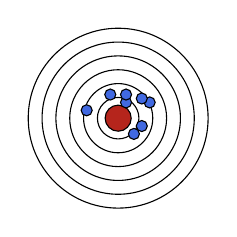
\begin{tikzpicture}
      \node[circle, minimum size=2, draw, fill=BrickRed] at (0, 0) {};
      \node[circle, minimum size=15, draw] at (0, 0) {};
      \node[circle, minimum size=25, draw] at (0, 0) {};
      \node[circle, minimum size=35, draw] at (0, 0) {};
      \node[circle, minimum size=45, draw] at (0, 0) {};
      \node[circle, minimum size=55, draw] at (0, 0) {};
      \node[circle, minimum size=65, draw] at (0, 0) {};

       \draw[fill=RoyalBlue] (0.4, 0.2) circle (2pt);
       \draw[fill=RoyalBlue] (-0.1, 0.3) circle (2pt);
       \draw[fill=RoyalBlue] (0.1, 0.2) circle (2pt);
       \draw[fill=RoyalBlue] (0.3, -0.1) circle (2pt);
       \draw[fill=RoyalBlue] (0.2, -0.2) circle (2pt);
       \draw[fill=RoyalBlue] (-0.4, 0.1) circle (2pt);
       \draw[fill=RoyalBlue] (0.1, 0.3) circle (2pt);
       \draw[fill=RoyalBlue] (0.3, 0.25) circle (2pt);
    \end{tikzpicture}     
    \caption{Biais faible, variance faible}
  \end{subfigure} \hfill
  \begin{subfigure}[t]{0.4\textwidth}
    \centering
    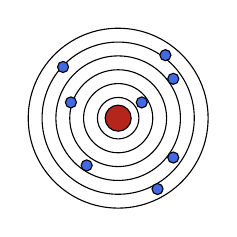
\begin{tikzpicture}
      \node[circle, minimum size=2, draw, fill=BrickRed] at (0, 0) {};
      \node[circle, minimum size=15, draw] at (0, 0) {};
      \node[circle, minimum size=25, draw] at (0, 0) {};
      \node[circle, minimum size=35, draw] at (0, 0) {};
      \node[circle, minimum size=45, draw] at (0, 0) {};
      \node[circle, minimum size=55, draw] at (0, 0) {};
      \node[circle, minimum size=65, draw] at (0, 0) {};

      \draw[fill=RoyalBlue] (0.6, 0.8) circle (2pt);
      \draw[fill=RoyalBlue] (-0.7, 0.65) circle (2pt);
      \draw[fill=RoyalBlue] (-0.4, -0.6) circle (2pt);
      \draw[fill=RoyalBlue] (0.5, -0.9) circle (2pt);
      \draw[fill=RoyalBlue] (0.7, -0.5) circle (2pt);
      \draw[fill=RoyalBlue] (-0.6, 0.2) circle (2pt);
      \draw[fill=RoyalBlue] (0.3, 0.2) circle (2pt);
      \draw[fill=RoyalBlue] (0.7, 0.5) circle (2pt);
    \end{tikzpicture}
    \caption{Biais faible, variance �lev�e}
  \end{subfigure}
  \begin{subfigure}[t]{0.4\textwidth}
    \centering
    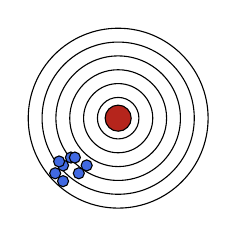
\begin{tikzpicture}
      \node[circle, minimum size=2, draw, fill=BrickRed] at (0, 0) {};
      \node[circle, minimum size=15, draw] at (0, 0) {};
      \node[circle, minimum size=25, draw] at (0, 0) {};
      \node[circle, minimum size=35, draw] at (0, 0) {};
      \node[circle, minimum size=45, draw] at (0, 0) {};
      \node[circle, minimum size=55, draw] at (0, 0) {};
      \node[circle, minimum size=65, draw] at (0, 0) {};

      \draw[fill=RoyalBlue] (-0.7, -0.6) circle (2pt);
      \draw[fill=RoyalBlue] (-0.6, -0.5) circle (2pt);
      \draw[fill=RoyalBlue] (-0.75, -0.55) circle (2pt);
      \draw[fill=RoyalBlue] (-0.5, -0.7) circle (2pt);
      \draw[fill=RoyalBlue] (-0.4, -0.6) circle (2pt);
      \draw[fill=RoyalBlue] (-0.8, -0.7) circle (2pt);
      \draw[fill=RoyalBlue] (-0.7, -0.8) circle (2pt);
      \draw[fill=RoyalBlue] (-0.55, -0.5) circle (2pt);
     \end{tikzpicture}
    \caption{Biais �lev�, variance faible}
  \end{subfigure} \hfill
  \begin{subfigure}[t]{0.4\textwidth}
    \centering
    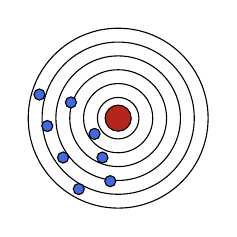
\begin{tikzpicture}
      \node[circle, minimum size=2, draw, fill=BrickRed] at (0, 0) {};
      \node[circle, minimum size=15, draw] at (0, 0) {};
      \node[circle, minimum size=25, draw] at (0, 0) {};
      \node[circle, minimum size=35, draw] at (0, 0) {};
      \node[circle, minimum size=45, draw] at (0, 0) {};
      \node[circle, minimum size=55, draw] at (0, 0) {};
      \node[circle, minimum size=65, draw] at (0, 0) {};

      \draw[fill=RoyalBlue] (-0.2, -0.5) circle (2pt);
      \draw[fill=RoyalBlue] (-1., 0.3) circle (2pt);
      \draw[fill=RoyalBlue] (-0.1, -0.8) circle (2pt);
      \draw[fill=RoyalBlue] (-0.5, -0.9) circle (2pt);
      \draw[fill=RoyalBlue] (-0.9, -0.1) circle (2pt);
      \draw[fill=RoyalBlue] (-0.6, 0.2) circle (2pt);
      \draw[fill=RoyalBlue] (-0.3, -0.2) circle (2pt);
      \draw[fill=RoyalBlue] (-0.7, -0.5) circle (2pt);
    \end{tikzpicture}
    \caption{Biais �lev�, variance �lev�e}
  \end{subfigure}
  \caption{Illustration des concepts de biais et de variance par analogie avec
    un jeu de fl�chettes. La quantit� � estimer est le centre de la cible ; les
    fl�chettes sont les estimations. Chacune des sous-figures pr�sente un
    estimateur diff�rent.}
  \label{fig:flechettes}
\end{figure}


\subsection{Convergence d'un estimateur $\bullet$}
\label{sec:convergence_estimateur}
On souhaite aussi d'un estimateur qu'il permette de s'approcher d'autant mieux
de la quantit� qu'il estime que la taille de l'�chantillon est grande. On parle
ici de la convergence d'une s�rie de variables al�atoires r�elles,
$(\Theta_n)_{n \in \NN^*},$ vers une valeur r�elle, $\theta$ ; il s'agit donc
en fait de consid�rer la convergence vers une variable al�atoire $\Theta$ qui
vaut $\theta$ presque partout.

On dit que l'estimateur $\Theta_n$ de $\theta$ \textbf{est convergent} s'il
converge en probabilit� vers $\theta:$
\begin{equation}
  \label{eq:estimateur_convergent}
  (\Theta_n)_{n \in \NN^*} \cvproba \theta.
\end{equation}

Si de plus la convergence est presque s�re,
$(\Theta_n)_{n \in \NN^*} \cvps \theta,$ on dit alors que $\Theta_n$ est un
estimateur \textbf{fortement convergent} de $\theta$.

\paragraph{Proposition} Un estimateur sans biais et de variance
asymptotiquement nulle est convergent.

\paragraph{Preuve} La preuve en a �t� faite dans l'exercice � Convergence vers
une constante � de Probabilit� IV. Pour rappel, posons $\Theta_n$ un estimateur
non biais� et de variance asymptotiquement nulle de $\theta \in \RR$,
c'est-�-dire que $\EE(\Theta_n) = \theta$ et $\VV(\Theta_n) \cvn 0.$ $\Theta_n$
est donc d'esp�rance et de variance born�es et ainsi dans $\Lcal^2.$ Enfin,
$  \EE((\Theta_n - \theta)^2) = \VV(\Theta_n) + B(\Theta_n)^2,$
et donc $\EE((\Theta_n - \theta)^2) \cvn 0,$ ce qui signifie que
$\Theta_n \cvltwo \theta$ et donc $\Theta_n \cvproba \theta. \hfill \square$

\paragraph{Remarque} On utilise en anglais le terme de ``\textit{consistent}'',
ce qui conduit les francophones � parfois parler d'estimateur consistant plut�t
que convergent.

\subsection{Exercice (estimation de la moyenne)}
\label{sec:exo_proprietes}
Nous cherchons � d�terminer le poids moyen des b�b�s � la naissance en
France. Pour cela, nous disposons d'un �chantillon $(x_1, x_2, \dots, x_n)$ de
$n$ mesures obtenues dans plusieurs maternit�s � travers le pays.

Nous supposons que cet �chantillon est une r�alisation d'un �chantillon
$(X_1, X_2, \dots, X_n)$ de variables al�atoire r�elles ind�pendantes et
identiquement distribu�es, d'esp�rance $m$ et de variance $\sigma^2$.

On propose deux estimateurs de $m$ : 
\[
  M_n = \frac1n \sum_{i=1}^n X_i \text{ et } Z_n = \frac12 (X_n + X_{n-1}).
\]

Montrer que $M_n$ et $Z_n$ sont sans biais. Lequel choisir pour approcher $m$ ?

(Solution : section~\ref{sec:sol_proprietes}.)


%-*- coding: iso-latin-1 -*-
\section{QCM}

\paragraph{Question 1.} Soit $X$ une variable al�atoire r�elle suivant une loi
de Poisson de param�tre $\lambda$. �tant donn� un �chantillon al�atoire
$(X_1, X_2, \dots, X_n)$ de $X$, et une de ses r�alisations
$(x_1, x_2, \dots, x_n)$, cocher le(s) estimateur(s) non biais�(s) de $\lambda$
parmi les propositions ci-dessous :
\begin{itemize}
\item[$\square$] $L_1 = \frac1n \sum_{i=1}^n x_i.$
\item[$\square$] $L_2 = \frac1n \sum_{i=1}^n X_i.$
\item[$\square$] $L_3 = \frac1n \sum_{i=1}^n \left( X_i^2 - \left( \frac1n \sum_{j=1}^n X_j \right)^2 \right).$
\item[$\square$] $L_4 = \frac1n \sum_{i=1}^n \left( x_i^2 - \left( \frac1n \sum_{j=1}^n x_j \right)^2 \right).$
\end{itemize}


\paragraph{Indice.}
{%
\noindent
\rotatebox[origin=c]{180}{%
\noindent
\begin{minipage}[t]{\linewidth}
Quelles sont l'esp�rance et la variance d'une loi de Poisson de param�tre $\lambda$ ?
\end{minipage}%
}%

\paragraph{Question 2.} Un estimateur biais� peut �tre plus pr�cis qu'un estimateur non-biais�.
\begin{itemize}
\item[$\square$] Vrai.
\item[$\square$] Faux.
\end{itemize}


\section*{Solution}
{%
\noindent
\rotatebox[origin=c]{180}{%
\noindent
\begin{minipage}[t]{\linewidth}
\paragraph{Question 1.} Il y a ici tout d'abord une question de vocabulaire :
un estimateur est une variable al�atoire, tandis qu'une estimation est sa
r�alisation. Ainsi nous ne consid�rons que les formules avec $X$ et non pas
avec $x$.

On rappelle que $\EE(X) = \lambda$ et $\VV(X) = \lambda.$

Seul $L_2$ est un estimateur sans biais de $\EE(X) = \lambda$ : c'est la moyenne
empirique de $X$.

On peut refaire le calcul : les $X_i$ �tant i.i.d. de m�me loi que $X,$ 
\[
  \text{B}(L_2) = \EE(L_2) - \lambda = \frac1n \sum_{i=1}^n \EE(X_i) - \lambda = 0.
\]

$L_3$ est la variance empirique de $X$ et $L_3$ est donc un estimateur
biais� de $\VV(X) = \lambda$. \newline

\paragraph{Question 2.} Vrai. C'est le concept du compromis biais-variance
(cf. section 3.4.3 du poly).
\end{minipage}%
}%

%%% Local Variables:
%%% mode: latex
%%% TeX-master: "../../sdd_2021_poly"
%%% End:




\section{Estimation par maximum de vraisemblance}
Nous consid�rons toujours dans cette section un �chantillon al�atoire
$(X_1, X_2, \dots, X_n)$ de taille $n \in \NN^*$ d'une variable al�atoire
r�elle $X$, et une quantit� $\theta \in \Scal \subseteq \RR$ � estimer. Nous
notons $\PP_X$ la loi de $X$.

Nous venons de voir comment caract�riser un estimateur $\Theta_n$ afin de
choisir le meilleur estimateur parmi plusieurs. Mais comment \textit{proposer} un
estimateur de $\theta$ ?

Supposons que $(x_1, x_2, \dots, x_n)$ est une r�alisation de
$(X_1, X_2, \dots, X_n)$. La technique que nous allons voir consiste �
maximiser la vraisemblance de l'�chantillon, autrement dit la probabilit�
d'observer cet �chantillon �tant donn�e la valeur estim�e de $\theta$.

\begin{exemple}
  Nous nous int�ressons � la r�ussite d'�l�ves au baccalaur�at en
  \^Ile-de-France, et disposons d'observations issues de plusieurs lyc�es de la
  r�gion.

  Nous mod�lisons l'observation \og r�ussite \fg~ou \og �chec \fg~comme la
  r�alisation d'une variable al�atoire $X$, de domaine $E = \{0, 1\}$ ($0$
  correspondant � \og �chec \fg~et $1$ � \og r�ussite \fg), et suivant une loi
  de probabilit� $\PP_X$.  Un choix classique pour cette loi de probabilit� est
  d'utiliser une loi de Bernoulli de param�tre $p$,:
  \[
    \PP_X(X=x) = p^x (1-p)^{1-x}.
  \] 
  Nos observations constituent un �chantillon
  $(x_1, x_2, \dots, x_n)$, qui est une r�alisation de l'�chantillon al�atoire
  $(X_1, X_2, \dots, X_n)$ de composantes ind�pendantes et identiquement
  distribu�es de m�me loi que $X$.

  Nous cherchons � estimer $p$ � partir de cet �chantillon. 

  Supposons que notre �chantillon contient $n=500$ �l�ves, dont $b=450$ ont
  eu le bac.

  La valeur $p=50\%$ est peu vraisemblable ; la valeur $p=90\%$ l'est beaucoup
  plus. C'est cette notion que nous allons formaliser par la suite.
\end{exemple}

La \textbf{vraisemblance} de l'�chantillon $(x_1, x_2, \dots, x_n)$ quantifie �
quel point il est plausible d'observer cet �chantillon en fonction de la valeur
de la quantit� � estimer.

Pour tout $t \in \Scal$, nous notons $\PP_{X; t}$ la loi de $X$ param�tr�e par
$t.$ Supposons qu'il existe une mesure $\mu$ sur $(\RR, \Bcal(\RR))$ telle que
$\PP_{X; t}$ s'�crive sous la forme $\PP_{X; t}= f_t \mu,$ o�
$f_t: \RR \mapsto \RR_+$ est $\mu$-mesurable. Dans le cas o� $X$ est discr�te,
$\mu$ est la mesure de comptage et $f_t$ la fonction de masse de $X$. Dans le
cas o� $X$ est � densit�, $\mu$ est la mesure de Lebesgue et $f_t$ est la
densit� de $X$. (Voir par exemple la section � Probabilit�s -- cadre g�n�ral �
de Probabilit�s III.) La vraisemblance de $(x_1, x_2, \dots, x_n)$ est alors la
fonction de $t$ d�finie par
\begin{equation}
  L(x_1, x_2, \dots, x_n; t) = \prod_{i=1}^n f_t(x_i).
  \label{eq:likelihood}
\end{equation}

Notez que la loi de l'�chantillon al�atoire $(X_1, X_2, \dots, X_n)$ est 
$  \PP_{X_1, X_2, \dots, X_n ; t} = \prod_{i=1}^n \PP_{X; t} $
car les $X_i$ sont ind�pendantes et identiquement distribu�es.

On appelle alors \textbf{estimation par maximum de vraisemblance} ({\it maximum
  likelihood estimate} ou {\it MLE} en anglais) de $\theta$ une valeur
$\hatmle{\theta}$ qui maximise la vraisemblance de l'�chantillon
$(x_1, x_2, \dots, x_n)$:
\begin{equation}
  \label{eq:mle_estimator}
  \hatmle{\theta} \in \argmax_{t \in \Scal} \prod_{i=1}^n f_t(x_i).
\end{equation}

\textbf{Un estimateur par maximum de vraisemblance} de $\theta$ est une
variable al�atoire r�elle $\hatmle{\Theta}$ dont la valeur quand
$X_1=x_1, X_2=x_2, \dots, X_n=x_n$ est donn�e par $\hatmle{\theta}$.

Pour simplifier les calculs, on choisira souvent de maximiser non pas
directement la vraisemblance mais son logarithme :
\begin{equation}
  \label{eq:lmle_estimator} 
  \hatmle{\theta} \in \argmax_{t \in \Scal}\sum_{i=1}^n \ln f_t(x_i).
\end{equation}

\begin{exemple}
  Reprenons notre exemple de r�ussite au baccalaur�at.
  
  L'estimation par maximum de vraisemblance de $p$ est
  \begin{align*}
    \hatmle{p} & = \argmax_{t \in [0, 1]} \sum_{i=1}^n \ln \PP_{X; t}(X=x_i)
                          = \argmax_{t \in [0, 1]} \sum_{i=1}^n \ln 
                          \left( t^{x_i} (1-t)^{1-x_i}  \right) \\
                        & = \argmax_{t \in [0, 1]} \sum_{i=1}^n x_i \ln t + 
                          \left( n - \sum_{i=1}^n x_i \right) \ln (1-t).
  \end{align*}
  La fonction
  $\ell: t \mapsto \sum_{i=1}^n x_i \ln t + \left( n - \sum_{i=1}^n x_i \right)
  \ln (1-t)$
  est concave, nous pouvons donc la maximiser en annulant sa d�riv�e :
  \begin{equation*}
    \frac{d \ell}{d t} = \sum_{i=1}^n x_i \frac1t - 
    \left( n - \sum_{i=1}^n x_i \right) \frac1{1-t},
  \end{equation*}
  ce qui nous donne
  \begin{equation*}
    (1 - \hatmle{p}) \left( \sum_{i=1}^n x_i \right) - \hatmle{p} \left( n - 
      \sum_{i=1}^n x_i \right) = 0
  \end{equation*}
  et donc
  \begin{equation}
    \label{eq:mle_bernoulli}
    \hatmle{p} = \frac{1}{n} \sum_{i=1}^n x_i = \frac{b}{n}.
  \end{equation}
  
  L'estimateur par maximum de vraisemblance de $p$ est ainsi tout simplement la
  moyenne empirique de l'�chantillon. Dans notre exemple, $p=450/500=90\%.$

  Remarque : en toute rigueur, on traitera s�par�ment les cas particuliers o� $\sum_{i=1}^n x_i=n$ ou $\sum_{i=1}^n x_i=0$.
\end{exemple}


\paragraph{Propri�t� $\bullet$} L'estimateur par maximum de vraisemblance est
(sous des hypoth�ses g�n�ralement v�rifi�es) convergent. La d�monstration,
plut�t p�nible, repose sur l'application de la loi des grands nombres : le
param�tre maximisant la vraisemblance maximise aussi la log-vraisemblance ainsi
que la log-vraisemblance divis�e par $n$.

\subsection{Exercice} 
\label{sec:rayleigh_exo}
Soit $X$ une variable al�atoire r�elle dont la densit� de probabilit� est donn�e par 
\[
  f(x; \sigma^2) = \frac{x}{\sigma^2} \exp \left( - \frac{x^2}{2 \sigma^2} \right) \text{ pour } x \in [0, +\infty[.
\]
On pourra v�rifier\footnote{Par exemple sur \href{https://fr.wikipedia.org/wiki/Loi_de_Rayleigh}{https://fr.wikipedia.org/wiki/Loi\_de\_Rayleigh}.} qu'il s'agit d'une loi de Rayleigh de param�tre d'�chelle
$\lambda = \sqrt{2} \sigma$. Ainsi son esp�rance et sa variance sont donn�es par 
\[
  \EE(X) = \sqrt{\frac{\pi}{2}} \sigma \text{\qquad et \qquad} \VV(X) =
  \frac{4-\pi}{2} \sigma^2.
\]
Donner l'estimateur par maximum de vraisemblance de $\sigma^2$.
Solution : voir section~\ref{sec:rayleigh_sol}.


\section{Estimation de Bayes $\bullet$}
\label{sec:bayes_est}
Supposons que plut�t que de ne pas conna�tre du tout la valeur du param�tre
$\theta$, nous ayons une bonne id�e des valeurs qu'il peut prendre. Cette
information peut �tre tr�s utile, surtout quand le nombre d'observations est
faible.

Pour en tirer parti, nous allons utiliser une variable al�atoire r�elle
$\Theta$ � valeurs dans $\Scal$, dont la loi $\PP_{\Theta}$ est la \textbf{loi
  a priori}, c'est-�-dire d�finie avant d'avoir observ� un �chantillon. Il va
maintenant s'agir d'utiliser la formule de Bayes pour exprimer la \textbf{loi a
  posteriori}, c'est-�-dire conditionnellement � un �chantillon al�atoire, de
$\Theta$.

Si $\Theta$ est discr�te, la formule de Bayes nous permet
d'�crire la loi de $\Theta|X_1, X_2, \dots, X_n :$
\begin{equation}
  \label{eq:bayes_discret}
  \PP_{\Theta|X_1, X_2, \dots, X_n}(\Theta=t) = \frac{\PP_{\Theta}(t) \prod_{i=1}^n f_t(x_i)}{
    \sum_{u \in \Scal} \PP_{\Theta}(u) \prod_{i=1}^n f_u(x_i)}
\end{equation}

Si $\Theta$ est � densit�, de densit� $g_{\Theta},$ alors
$\Theta|X_1, X_2, \dots, X_n$ est aussi � densit� et la formule de Bayes nous
permet d'�crire sa densit� comme : 
\begin{equation}
  \label{eq:bayes_densite}
  g_{\Theta|X_1, X_2, \dots, X_n}(\Theta=t) = \frac{g_{\Theta}(t) \prod_{i=1}^n f_t(x_i)}{
    \int_{\Scal} g_{\Theta}(u) \prod_{i=1}^n f_u(x_i) du}
\end{equation}
Ces manipulations de Bayes sont analogues � celles effectu�es dans le poly de
Probabilit�s III, en particulier dans la section � Formule de balayage
conditionnel � et dans l'exercice � Loi conjugu�es �.

En d'autres termes, l'observation d'un �chantillon permet d'ajuster la loi a
priori de $\Theta$ en sa loi a posteriori. Cette id�e est au c\oe{}ur
de \textbf{l'inf�rence bay�sienne.}


L'estimation de Bayes de $\theta$ est d�finie comme une valeur de $\Scal$ qui
est la mieux estim�e par la loi a posteriori de $\Theta$. Cette d�finition est
g�n�rale, et d�pend du sens donn� � � mieux estim�e par � ; nous utiliserons
une des d�finitions les plus courantes, et consid�rons � partir de maintenant
l'erreur quadratique moyenne (d�finie section~\ref{sec:precision_estimateur}). 

L'\textbf{estimation de Bayes pour l'erreur quadratique moyenne} de $\theta$
est ainsi d�finie par
\begin{equation}
  \label{eq:bayes_estimator}
  \hatbys{\theta} \in \argmin_{t \in \Scal} \EE([(\Theta|X_1=x_1, X_2=x_2, \dots, X_n=x_n) - t)]^2).
\end{equation}


\paragraph{Propri�t�} L'estimation de Bayes pour l'erreur quadratique moyenne
est l'esp�rance de la distribution a posteriori de $\Theta$ : 
\begin{equation}
  \label{eq:bayes_estimator2}
  \hatbys{\theta}  = \EE(\Theta|X_1 = x_1, X_2=x_2, \dots, X_n=x_n).
\end{equation}

\paragraph{Preuve}
En effet, posons $t \in \Scal.$ Notons
$W = (\Theta|X_1=x_1, X_2=x_2, \dots, X_n=x_n)$ pour simplifier l'�criture.
Alors
\begin{equation*}
  \EE((W - t)^2) =  \EE(W^2) + t^2 - 2 t \EE(W) =  \EE(W^2) + [\EE(W) - t]^2 - \EE(W)^2.  
\end{equation*}
Comme ni $\EE(W^2)$ ni $\EE(W)^2$ ne d�pendent de $t,$
$\hatbys{\theta}$ est obtenue en minimisant $(\EE(W) - t)^2$ et donc $\hatbys{\theta} = 
\EE(W). \hfill \square$

\begin{exemple}
  Reprenons notre exemple de taux de r�ussite au baccalaur�at.  Nous supposons
  maintenant que $p$ est une r�alisation d'une variable al�atoire $\Theta$ qui
  suit une loi b�ta de param�tres $(\alpha, \beta)$
  (cf. section~\ref{sec:loi_beta}).

  Pour calculer l'estimateur de Bayes de $p$, il nous faut conna�tre la loi
  \[
    \PP(\Theta|X_1=x_1, X_2=x_2, \dots, X_n=x_n).
  \]
  
  La loi de Bayes, combin�e � l'hypoth�se d'ind�pendance et de distribution
  identique des $X_i$, nous permet d'�crire
  \begin{flalign*}
     & \PP(\Theta=p|X_1=x_1, \dots, X_n=x_n)  = \frac{\PP(X_1=x_1, \dots, X_n=x_n|p) \PP(p)}{\PP(X_1=x_1, \dots, X_n=x_n)} \\
    & = \frac{1}{\PP(X_1=x_1, \dots, X_n=x_n) B(\alpha, \beta)} 
    \prod_{i=1}^{n} p^{x_i} (1-p)^{1-x_i}  p^{\alpha-1}
    (1-p)^{\beta-1} \\
    & = \frac{1}{\PP(X_1=x_1, \dots, X_n=x_n) B(\alpha, \beta)} 
    p^{b + \alpha - 1} (1-p)^{n - b + \beta - 1}. 
  \end{flalign*}
  
  On reconna�t ici la densit� d'une nouvelle loi b�ta.  Ainsi
  $(\Theta|X_1=x_1, \dots, X_n=x_n)$ suit une loi b�ta de param�tres $(b + \alpha)$ et
  $(n - b + \beta).$

  L'estimation de Bayes de $p$ est ainsi
  \begin{equation*}
    \hatbys{p} = \EE(\Theta|X_1=x_1, X_2=x_2, \dots, X_n=x_n) = \frac{(b + \alpha)}{
      (b + \alpha) + (n - b + \beta)}
    = \frac{b + \alpha}{n + \alpha + \beta}.
  \end{equation*}
  Cette premi�re �galit� est obtenue d'apr�s la formule donnant l'esp�rance
  d'une loi b�ta (cf section~\ref{sec:loi_beta}).

  \textbf{Remarque importante}
  On peut r��crire cette estimation sous la forme
  \begin{equation*}
    \hatbys{p} = \frac{\alpha + \beta}{n + \alpha + \beta} \EE[\Theta] + 
    \frac{n}{n + \alpha + \beta} \hatmle{p}.
  \end{equation*}
  Ainsi, l'estimation de Bayes du param�tre $p$ est une combinaison lin�aire de
  l'esp�rance de sa distribution a priori et de son estimation par maximum de
  vraisemblance.

  De plus, le coefficient multiplicatif de l'esp�rance a priori d�cro�t en
  fonction de la taille $n$ de l'�chantillon, tandis que le coefficient
  multiplicatif de l'estimation par maximum de vraisemblance cro�t en fonction
  de $n$. Ainsi, plus l'�chantillon est grand, plus l'estimateur de Bayes fait
  confiance aux donn�es, et s'�loigne de l'esp�rance a priori du param�tre,
  dont on est plus proche avec un petit �chantillon.

  La figure~\ref{fig:bayes_estimate} illustre cet exemple.

  \textbf{Remarque} Le choix d'une loi b�ta ne s'est pas fait au hasard. On
  retrouve ici les lois conjugu�es pr�sent�es en exercice de Probabilit�s
  III. En inf�rence bay�sienne, on dit qu'une loi a priori et une loi a
  posteriori sont conjugu�es lorsqu'elles appartiennent � la m�me famille. En
  particulier, la loi b�ta est conjugu�e � elle-m�me pour une vraisemblance de
  Bernoulli.
\end{exemple}

\begin{figure}[h]
  \centering
  \includegraphics[width=\textwidth]{figures/estimation/bayes_estimate}
  \caption{Loi a priori et a posteriori pour le param�tre $p$ dans l'exemple du
    taux de r�ussite au baccalaur�at. Sans voir de donn�es, $p=0,80$,
    c'est-�-dire l'esp�rance de sa loi a priori (croix bleue). En utilisant
    uniquement l'�chantillon, $p=0,90$, c'est-�-dire son estimation par maximum
    de vraisemblance (triangle vert). L'estimation de Bayes (rond orange) est
    interm�diaire.}
  \label{fig:bayes_estimate}
\end{figure}




\section{Compl�ments}
\subsection{Variance de la moyenne empirique} 
\label{sec:variance_moyenne_empirique}

Soit $X$ une variable al�atoire
r�elle de carr� int�grable, d'esp�rance $m$ et de variance $\sigma^2$. Soient
$X_1, X_2, \dots, X_n$ ind�pendantes et identiquement distribu�es, de m�me loi
que $X$. 

Par d�finition de la variance, $\sigma^2 = \EE(X^2) - \EE(X)^2$ donc
$\EE(X^2) = \sigma^2 + m^2$.

Posons $M_n = \frac1n \sum_{i=1}^n X_i.$
\begin{align*}
  \VV(M_n) &= \EE(M_n^2) - \EE(M_n)^2 
   = \EE\left(\left(\frac1n \sum_{i=1}^n X_i\right)^2\right) - m^2 
   = \frac1{n^2} \EE\left( \sum_{i=1}^n X_i \sum_{j=1}^n X_j\right) - m^2 \\
  & = \frac1{n^2} \EE\left( \sum_{i=1}^n \left(X_i^2 + \sum_{j \neq i }^n X_i X_j \right) \right) - m^2 
   = \frac1{n} \left(\EE(X^2) + \sum_{j \neq i }^n \EE(X)^2 \right) - m^2, 
\end{align*}
par lin�arit� de l'esp�rance et car, pour $i \neq j$, $X_i$ et $X_j$ sont ind�pendantes et donc $\EE(X_iX_j) = \EE(X_i) \EE(X_j) = \EE(X)^2.$
Ainsi,
\[
  \VV(M_n) = \frac1{n} \left(\underbrace{\sigma^2 + m^2}_{\EE(X^2)} + (n-1) \, \underbrace{m^2}_{\EE(X)^2}  \right) - m^2 = \frac{\sigma^2}{n}.
\]

\subsection{Biais de la variance empirique} 
\label{sec:biais_variance_empirique}
Soit $X$ une variable al�atoire
r�elle de carr� int�grable, d'esp�rance $m$ et de variance $\sigma^2$. Soient
$X_1, X_2, \dots, X_n$ ind�pendantes et identiquement distribu�es, de m�me loi
que $X$. 

Posons $M_n = \frac1n \sum_{i=1}^n X_i$ et $S_n = \frac1n \sum_{i=1}^n (X_i - M_n)^2.$ Alors
\begin{align*}
  \EE(S_n) = \frac1n \sum_{i=1}^n \EE((X_i - M_n)^2)  & =  
    \frac1n \sum_{i=1}^n \left( \EE(X_i^2) +  \EE(M_n^2) - 2 \EE(X_i M_n) \right)  \\
  & = \EE(X^2) + \EE(M_n^2) - \frac2n \sum_{i=1}^n \EE(X_i M_n).
\end{align*}
Nous avons montr� lors du calcul de la variance de la moyenne empirique (section~\ref{sec:variance_moyenne_empirique}) que
$\EE(X^2) = \sigma^2 + m^2$ et que $\EE(M_n^2) = m^2 + \frac{\sigma^2}{n}.$
De plus, par lin�arit� de l'esp�rance,
\[
  \EE(M_n^2) = \EE\left( \left(\frac1n \sum_{i=1}^n X_i \right) M_n \right) = \frac1n \sum_{i=1}^n \EE(X_i M_n),
\]
et donc 
\[
  \EE(M_n^2) - \frac2n \sum_{i=1}^n \EE(X_i M_n) = - \EE(M_n^2).
\]

On obtient ainsi 
\[
  \EE(S_n) = (\sigma^2 + m^2) - \left(m^2 + \frac{\sigma^2}{n}\right) = \frac{n-1}{n} \sigma^2.
\]
La variance empirique est donc biais�e et son biais vaut 
\[
  \text{B}(S_n) = \EE(S_n) - \sigma^2 = - \frac1n \sigma^2.
\]

\subsection{Solution de l'exercice~\ref{sec:exo_proprietes}}
\label{sec:sol_proprietes}
La d�monstration pour la moyenne empirique $M_n$ a �t� faite plus haut.

En ce qui concerne $Z_n$, 
\[
  \EE(Z_n) = \frac12 (\EE(X_n) + \EE(X_{n-1})) = m.
\]

Nous avons assez naturellement envie d'utiliser $M_n$, qui utilise toutes les
observations, plut�t que $Z_n$, qui n'en utilise que deux.

Pour nous en convaincre, nous pouvons comparer les variances de $M_n$ et
$Z_n$. La variance de la moyenne empirique est $\VV(M_n) = \frac{\sigma^2}{n}$
(voir plus haut). La variance de $Z_n$, elle, vaut
\[
  \VV(Z_n) = \frac14 \left( \VV(X_n) + \VV(X_{n-1}) \right) = \frac{\sigma^2}{2},
\]
la premi�re �galit� �tant obtenue par ind�pendance de $X_n$ et $X_{n-1}$.

$Z_n$ est ainsi un estimateur bien moins pr�cis que $M_n$ d�s que $n>2.$

\subsection{Loi Beta}
\label{sec:loi_beta}
La densit� de probabilit� de la {\it loi b�ta} de param�tres
$\alpha, \beta > 0$, d�finie sur $0 \leq u \leq 1$, est donn�e par :
\begin{equation}
  \label{eq:beta_distribution}
  f_{\alpha, \beta} (u) = \frac{u^{\alpha -1} (1-u)^{\beta-1}}{B(\alpha, \beta)}     
\end{equation}
o�
$B(\alpha, \beta) = \frac{\Gamma(\alpha) \Gamma(\beta)}{\Gamma(\alpha+\beta)}$
et $\Gamma$ est la fonction gamma. L'esp�rance de cette loi est
$\frac{\alpha}{\alpha + \beta}$.

\subsection{Solution de l'exercice~\ref{sec:rayleigh_exo}}
\label{sec:rayleigh_sol}
Soit $(x_1, x_2, \dots, x_n)$ un �chantillon de $X$ de taille $n \in \NN^*.$ La
log-vraisemblance de l'�chantillon est donn�e par
\[
  \ell(x_1, x_2, \dots, x_n; \sigma^2) = \sum_{i=1}^n \ln \left(
    \frac{1}{\sigma^2} x_i \exp\left(- \frac{x_i^2}{2\sigma^2} \right)\right) 
  = -n \ln(\sigma^2) + \sum_{i=1}^n \ln(x_i) - \frac{1}{2\sigma^2} \sum_{i=1}^n x_i^2.
\]
Ainsi, l'estimation par maximum de vraisemblance de $\sigma^2$ est donn�e par :
\[
  \hatmle{\sigma^2} \in \argmax_{s \in \RR_+} \left(-n \ln(s) + \sum_{i=1}^n \ln(x_i) - 
\frac{1}{2s} \sum_{i=1}^n x_i^2\right).
\]
On obtient un point critique de la fonction de $\RR_+$ dans $\RR$ qui � $s$
associe $-n \ln(s) + \sum_{i=1}^n \ln(x_i) - \frac{1}{2s} \sum_{i=1}^n x_i^2$
en annulant sa d�riv�e, qui vaut :
\[
  s \mapsto - \frac{n}{s} + \frac12 \sum_{i=1}^n x_i^2 \frac{1}{s^2},
\]
et donc 
\[
  \hatmle{\sigma^2} = \frac{1}{2n} \sum_{i=1}^n x_i^2.
\]
(On v�rifiera que ce point critique est bien un maximum.)
Ainsi, �tant donn� un �chantillon al�atoire $(X_1, X_2, \dots, X_n)$ de $X$,
l'estimateur par maximum de vraisemblance de $\sigma^2$ est donn� par
\[
  S_n = \frac{1}{2n} \sum_{i=1}^n X_i^2.
\]


\begin{plusloin}
\item Un exercice sur la fonction de r�partition empirique vous a �t� propos�
  dans le poly de Probabilit� III.
\item On peut construire un estimateur par la \textit{m�thode des moments}, qui
  consiste � faire coincider les moments th�oriques de $\PP_X$ (qui d�pendent
  donc de $\theta$) avec les moments empiriques de l'�chantillon. La loi des
  grands nombres justifie en effet d'approcher la moyenne par la moyenne
  empirique. Cette m�thode est g�n�ralement moins pr�cise que le maximum de
  vraisemblance.
\item Plus la variance d'un estimateur est faible, plus cet estimateur
  peut-�tre consid�r� comme pr�cis. La \textit{borne de Cram�r-Rao} est une
  borne inf�rieure de cette variance pour un estimateur sans biais, en se
  basant sur l'information de Fisher. On dit qu'un estimateur est
  \textit{efficace} s'il est non-biais� et que sa variance tend vers sa borne
  de Cram�r-Rao.
\end{plusloin}

%\clearpage
%-*- coding: iso-latin-1 -*-

\section{QCM}
\paragraph{Question 1.} Soit $(x_1, x_2, \dots, x_n)$ un �chantillon d'une
variable al�atoire $X$. On suppose que $X$ suit une loi param�tris�e
par $\gamma$. La vraisemblance de $(x_1, x_2, \dots, x_n)$ est donn�e par
\begin{itemize}
\item[$\square$] $\PP(x_1, x_2, \dots, x_n, \gamma)$
\item[$\square$] $\PP(x_1, x_2, \dots, x_n | \gamma)$
\item[$\square$] $\PP(\gamma | x_1, x_2, \dots, x_n)$
\item[$\square$] $\prod_{i=1}^n \PP(x_i|\gamma)$
\item[$\square$] $\prod_{i=1}^n \PP(\gamma|x_i)$
\end{itemize}

\paragraph{Question 2.} Soit $X$ une loi exponentielle de param�tre
$\lambda$. L'estimateur par maximum de vraisemblance de $\lambda$ est donn� par
\begin{itemize}
\item[$\square$] $L_n = n \ln(\lambda) - \lambda \sum_{i=1}^n X_i,$ o� $(X_1, X_2, \dots, X_n)$ est un �chantillon al�atoire de $X$
\item[$\square$] $\widehat{\lambda} = n \ln(\lambda) - \lambda \sum_{i=1}^n x_i,$ o� $(x_1, x_2, \dots, x_n)$ est un �chantillon al�atoire de $X$
\item[$\square$] $L_n = \frac{n}{\sum_{i=1}^n X_i},$ o� $(X_1, X_2, \dots, X_n)$ est un �chantillon al�atoire de $X$
\item[$\square$] $\widehat{\lambda} = \frac{n}{\sum_{i=1}^n x_i},$ o� $(x_1, x_2, \dots, x_n)$ est un �chantillon al�atoire de $X$.
\end{itemize}

\paragraph{Question 3. $\bigstar$} L'estimateur de Bayes est plus proche de l'esp�rance a
priori que de l'estimateur par maximum de vraisemblance quand la taille de
l'�chantillon est
\begin{itemize}
\item[$\square$] grande
\item[$\square$] petite
\item[$\square$] �a d�pend.
\end{itemize}



\section*{Solution}

{%
\noindent
\rotatebox[origin=c]{180}{%
\noindent
\begin{minipage}[t]{\linewidth}
\paragraph{Question 1.} Par d�finition (cf. �quation~(3.7) du poly),
\[
L(x_1, x_2, \dots, x_n; \gamma) = \PP(x_1, x_2, \dots, x_n | \gamma) = \prod_{i=1}^n \PP(x_i|\gamma).
\]

\paragraph{Question 2.} 
Par d�finition la vraisemblance d'un �chantillon $(x_1, x_2, \dots, x_n)$ est donn�e par
\[
  L(x_1, x_2, \dots, x_n; \lambda) = \prod_{i=1}^n \lambda e^{- \lambda x_i}
  = \lambda^n \prod_{i=1}^n e^{- \lambda x_i},
\] 
et donc sa \textit{log-vraisemblance} vaut 
\[
  \ell(x_1, x_2, \dots, x_n; \lambda) = \ln \left(\lambda^n \prod_{i=1}^n e^{- \lambda x_i}\right)
  = n \ln(\lambda) - \lambda \sum_{i=1}^n x_i.
\]
La fonction $\lambda \mapsto n \ln(\lambda) - \lambda \sum_{i=1}^n x_i$ est
concave sur $]0, +\infty[ \rightarrow \RR$ et on peut donc la maximiser en
annulant sa d�riv�e.

On obtient \textit{l'estimation par maximum de vraisemblance} de $\lambda$ suivante :
\[
  \hatmle{\lambda} = \frac{n}{\sum_{i=1}^n x_i}
\]
et, si on appelle $(X_1, X_2, \dots, X_n)$ un �chantillon al�atoire de $X$, on
obtient \textit{l'estimateur par maximum de vraisemblance} de $\lambda$ :
\[
  L_n = \frac{n}{\sum_{i=1}^n X_n}.
\]


\paragraph{Question 3.} La tendance que nous avons observ�e sur l'exemple de la
section 3.6 (cf. � Remarque importante �) se v�rifie en g�n�ral : plus on
observe d'�chantillons, plus on s'�loigne de l'a priori pour se rapprocher d'un
estimateur issu uniquement des donn�es.
\end{minipage}%
}%



%%% Local Variables:
%%% mode: latex
%%% TeX-master: "../sdd_2021_poly"
%%% End:



\clearpage

\chapter{Tests d'hypoth�se}
\input{contents/tests}

\part{Analyse exploratoire}
\vspace{1cm}
\chapter{R�duction de dimension}
\input{contents/dimred}
\clearpage 

\chapter{Bonnes pratiques}
\input{contents/pratiques}

\part{Apprentissage supervis�}
\chapter{Minimisation du risque empirique}
\input{contents/erm}
\clearpage 

\chapter{G�n�ralisation}
\input{contents/generalisation}
\clearpage 

\chapter{Mod�les non-lin�aires}
\input{contents/nonlin}
\clearpage 


\end{document}

%%% Local Variables:
%%% mode: latex
%%% TeX-master: t
%%% End:
